%%%% ijcai20.tex

\typeout{IJCAI--PRICAI--20 Instructions for Authors}

% These are the instructions for authors for IJCAI-20.

\documentclass{article}
\pdfpagewidth=8.5in
\pdfpageheight=11in
\usepackage{cite}
% The file ijcai20.sty is NOT the same than previous years'
\usepackage{ijcai20}

% Use the postscript times font!
\usepackage{times}
\usepackage{soul}
\usepackage{url}
\usepackage[hidelinks]{hyperref}
\usepackage[utf8]{inputenc}
\usepackage[small]{caption}
\usepackage{graphicx}
\usepackage{amsmath}
\usepackage{amsthm}
\usepackage{paralist}
\usepackage{booktabs}
\usepackage{algorithm}
\usepackage{algorithmic}
\urlstyle{same}
\newcommand{\ourtool}{\texttt{ZebraTutor}}

\newtheorem{example}{Example}
\newtheorem{theorem}{Theorem}

\title{ZebraTutor: Visual step-by-step explanations on how to solve Logic Grid Puzzles (Demo)}

\author{
Bart Bogaerts$^1$
\and
Emilio Gamba$^1$\and
Tias Guns$^1$
\affiliations
$^1$Vrije Universiteit Brussel\\
\emails
\{firstname.lastname\}@vub.be
}

\begin{document}
% The submitted document must be a single PDF. The paper should describe the application domain, the problem scenario, the technology used, the AI techniques involved, the original contribution and innovations of the system, live and interactive aspects, etc. Papers must be prepared in PDF format using the IJCAI style. Submissions are NOT anonymous. The page limit is 3 pages in total: 2 pages for the main text (including all figures but excluding references), and one additional page for references. Over-length papers will be rejected without review. 

\maketitle

\begin{abstract}
In this demonstration, we present \ourtool, an integrated solution for explaining how to solve constraint satisfaction problems, with a use case on logic grid puzzles. More precisely, we study the problem of explaining inference steps that one can take during propagation, in a way that is easy to interpret for a person. Consequently, we aim to give the constraint solver explainable agency, which can help in building trust in the solver by being able to understand and even learn from explanations.
For logic grid puzzles (also known as zebra puzzles), the challenge is to find a sequence of \textit{simple} explanations how the solution can be obtained from the clues. Furthermore, each explanation should aim to be as cognitively easy as possible for a human to verify and understand.
Through our tool, we present an approach, applied to logic grid puzzles, that is agnostic of the underlying constraint propagation mechanism, and that can provide explanations even for inference steps requiring combinations of constraints. The difficulty of an explanation is evaluated using a cost function. Our algorithm iteratively constructs the explanation sequence by using an optimistic estimate of the cost function to guide the search for the best explanation at each step.
An overview of this end-to-end solution is depicted on \ref{fig:infopipeline}.

\end{abstract}

\section{Introduction}


\ourtool\footnote{\ourtool follows-up from our demonstration presented at the BNAIC/BENELEARN conference and the publication entitled ``Step-wise explanations of constraint satisfaction problems''}~starts from a plain English language representation of the clues and a list of all entities present in the puzzle. It then applies NLP techniques to build a puzzle-specific lexicon. The lexicon is fed into a type-aware variant of the semantical framework of Blackburn \& Bos~[\citeyear{Blackburn2005,Blackburn2006}] which translates the clues into Discourse Representation Theory \cite{DRT}. This logic is further transformed to a specification in the IDP language, a typed extension of first-order logic.

It then uses this formal representation of clues to solve the puzzle and to explain how a user can find this solution. The focus of our explanation is on simplicity: in generating explanations and choosing the order in which the reasoning steps are explained, we chose to order by an estimate of mental effort required to follow the reasoning step. Each reasoning step is visualised as the clue(s) involved and the resulting changes on the grid.
Whenever we encounter an explanation step that is \textit{difficult enough}, meaning at least two constraints and at least some assumption are involved, we try to further break this explanation down into smaller explanation steps. Thus, for a difficult explanation step, we try to find a \textit{nested sequence} of explanations. 

For such propagations, with constraints $\{ C_1, ...,C_n\}$, and for each fact they propagate, we look for a contradiction-based sequence of propagations such that at every step in the propagation only a subset of all the constraints is used. If that is not possible, this would mean that the nested sequence contains a step that is as difficult as the original one. In other words, we could not find a nested sequence that would be easier to understand.

When solving such puzzles, it can either be used for explaining how to obtain an entire solution, or for providing help to users who are stuck during the solving process. Indeed, our explanation method will, given a partial solution, find the easiest next derivation to make.




\section{System Overview}
The input to \ourtool is a set of natural language sentences (from hereon referred to as ``clues''), and the names of the entities that make up the puzzle, e.g arrabiata sauce, farfalle, claudia, etc. \\
In typical logic grid puzzles, the entity names are present in the grid that is supplied with the puzzle. For some puzzles, not all entities are known or required to know in advance; a prototypical example is Einstein's Zebra puzzl, which ends with the question ``Who owns the zebra'', while the clues do not name the Zebra entitiy, and the puzzle can be solved without the knowledge of the fact that there is a zebra in the first place.



\paragraph{Steps} Our framework consists of the following steps, starting from the input:
\begin{compactenum}
        \item \textbf{Part-of-Speech (POS) tagging}: A part-of-speech tag is associated with each word using the NTLK perceptron tagger\cite{marcus1993building}.
        \item \textbf{Chunking and lexicon Building} : A problem-specific lexicon is constructed; each word or set of words(chunk) is assigned a role, based on the POS-tags.
        \item \textbf{Parsing}: We used a typed variant of the Blackburn and bos framework to use the lexicon and grammar to derive a logical formulation of the clues in Discourse Representation Theory.
        \item \textbf{From logic to complete IDP specification}: the logical representation is translated into the IDP language and augmented with logic-grid-specific information.
        \item \textbf{Explanation-producing search in IDP}: We exploit the IDP representation of the clues to find a sequence of \textit{simple} explanations, where each explanation should aim to be as cognitively easy as possible for a human to verify and understand. 
        \item \textbf{Visualisation of the explanation}: All explanation steps are visualised by means of a colour-coded logic grid, where different colours are used to highlight the existing facts, the new fact and the clue or inference technique used.
\end{compactenum}

\begin{figure*}[t]
    \centering
    
\includegraphics[width=\linewidth]{ijcaidemo-1.png}
    \caption{Overview of the processing steps from input to visualisation}
    \label{fig:infopipeline}
\end{figure*}
\section{Demonstration}
An online demo of our system can be found on \url{https://bartbog.github.io/zebra}, containing examples with an explanation of the information pipeline. This web page contains for some puzzles:
\begin{itemize}
    \item All entities with their corresponding entity types; 
    \item The logic grid used to fill in the facts derived from the clues;
    \item The clues and inference techniques (logigram constraints) used in the solving process.
    \item Each word of each clue sentence associated with a POS-tag.
    \item The lexicon that is required to parse the puzzles (semi-automatically generated).
    \item The resulting discourse representation theory and IDP theory associated to each of the clues.
    \item The visualisation of the explanation by derivation steps. 
\end{itemize}

\begin{figure}[H]
    \centering
    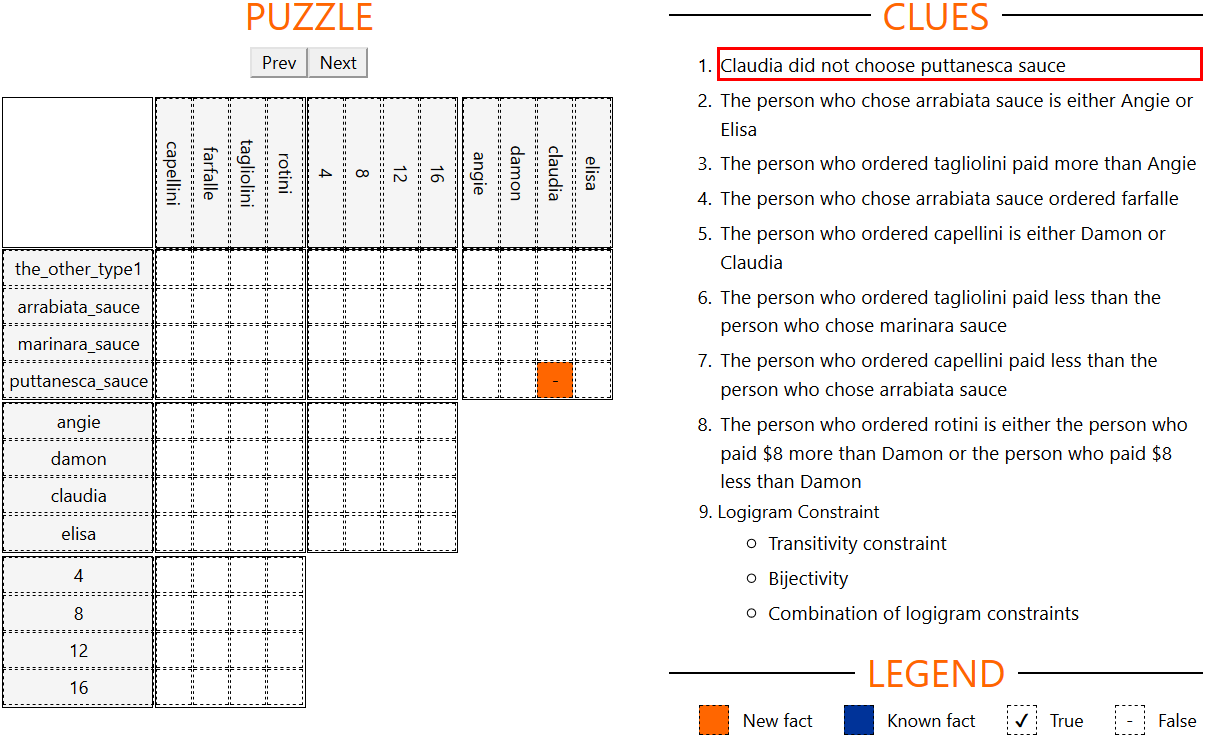
\includegraphics[width=\linewidth]{puzzle.png}
    \caption{Logic grid for the pasta puzzle}
    \label{fig:pasta_grid}
\end{figure}

The website is still under construction, and will be updated in the near future to allow for interaction with the logic grid and live explanations of next possible inference steps.
\clearpage
%% The file named.bst is a bibliography style file for BibTeX 0.99c
\bibliographystyle{named}
\bibliography{ijcai20}

\end{document}

